\documentclass[11pt]{article}
\usepackage[scaled=0.92]{helvet}
\usepackage{geometry}
\geometry{letterpaper,tmargin=1in,bmargin=1in,lmargin=1in,rmargin=1in}
\usepackage[parfill]{parskip} % Activate to begin paragraphs with an empty line rather than an indent %\usepackage{graphicx}
\usepackage{amsmath,amssymb, mathrsfs, dsfont}
\usepackage{mathtools}

\usepackage{tabularx}
\usepackage[font=footnotesize,labelfont=bf]{caption}
\usepackage{graphicx}
\usepackage{xcolor}
%\usepackage[linkbordercolor ={1 1 1} ]{hyperref}
%\usepackage[sf]{titlesec}
\usepackage{natbib}
\usepackage{../../Tianpei_Report}

%\usepackage{appendix}
%\usepackage{algorithm}
%\usepackage{algorithmic}

%\renewcommand{\algorithmicrequire}{\textbf{Input:}}
%\renewcommand{\algorithmicensure}{\textbf{Output:}}



\begin{document}
\title{Lecture 6: Temporal-Difference Learning}
\author{Tianpei Xie}
\date{ Aug 5th., 2022 }
\maketitle
\tableofcontents
\newpage
\section{Introduction}
If one had to identify one idea as \underline{central and novel} to reinforcement learning, it would undoubtedly be temporal-di↵erence (TD) learning \citep{sutton2018reinforcement}.  \textbf{\emph{Temporal-Difference (TD) Learning}} is a combination of Monte Carlo ideas and dynamic programming (DP) ideas. Like Monte Carlo methods, TD methods can learn directly from raw experience \underline{without a model of the}  \underline{environment’s dynamics}. Like DP, TD methods update estimates based in part on other learned estimates, without waiting for a final outcome (they \underline{bootstrap}). The relationship between TD, DP, and Monte Carlo methods is a recurring theme in the theory of reinforcement learning. 

Note that TD, DP, and Monte Carlo \emph{control} all use the same Generalized Policy Iteration (GPI) methods to improve policy. The differences in the methods are primarily differences in their approaches to the \emph{prediction} problem.

Another thing to note is that all of methods we discussed above is  Tabular method, since we do not assume any functional form for the value function but just record it into a table. 
\section{Temporal-Difference Prediction}
Recall that in Monte Carlo Methods, the value function is estimated by sample episodes. We can write it into an \emph{incremental update}. Let $V(s)$ be the (empirical) estimate of state-value $v_{\pi}(s)$,  
\begin{align*}
v_{\pi}(s) &= \E{\pi}{G_{t} | S_{t} = s} \\
&\approx \E{\text{emp}}{G_{t} | S_{t} = s} := V_{N(s)}(s)  \\
&= \frac{\sum_{t=1}^{N(s)} G_{t}}{N(s)}\, \\
&= \frac{1}{N(s)}\brac{G_{N(s)} + (N(s)-1)\frac{\sum_{t=1}^{N(s)-1} G_{t}}{N(s)-1}} \\
&= \frac{\sum_{t=1}^{N(s)-1} G_{t}}{N(s)-1} + \frac{1}{N(s)}\brac{G_{N(s)} -  \frac{\sum_{t=1}^{N(s)-1} G_{t}}{N(s)-1}} \\
V_{N(s)}(s)&= V_{N(s)-1}(s) + \alpha_{N(s)}\brac{G_{N(s)} -  V_{N(s)-1}(s) }
\end{align*} where $N(s) = |T(s)|$ and $T(s) = \{S_{t}=s\}_{t=1}^{\infty}$ or the number of epsiodes for first-visit MC. The above incremental update can be summarized as \begin{align}
V(S_{t}) &\leftarrow V(S_{t}) + \alpha_{t}\paren{G_{t} - V(S_{t})} \label{eqn: incremental_update}\\
\text{\textbf{new} estimate}&\leftarrow \text{\textbf{old} estimate} + \text{step\_size}\paren{\text{\textbf{target}} - \text{\textbf{old} estimate}} \nonumber
\end{align} This formula defines the value function using two terms: the \textbf{old estimate}, and the \textbf{difference} between the target and the old estimate. We call this algorithm\emph{ constant-$\alpha$ Monte Carlo}. 

\begin{figure}
\begin{minipage}[t]{1\linewidth}
  \centering
  \centerline{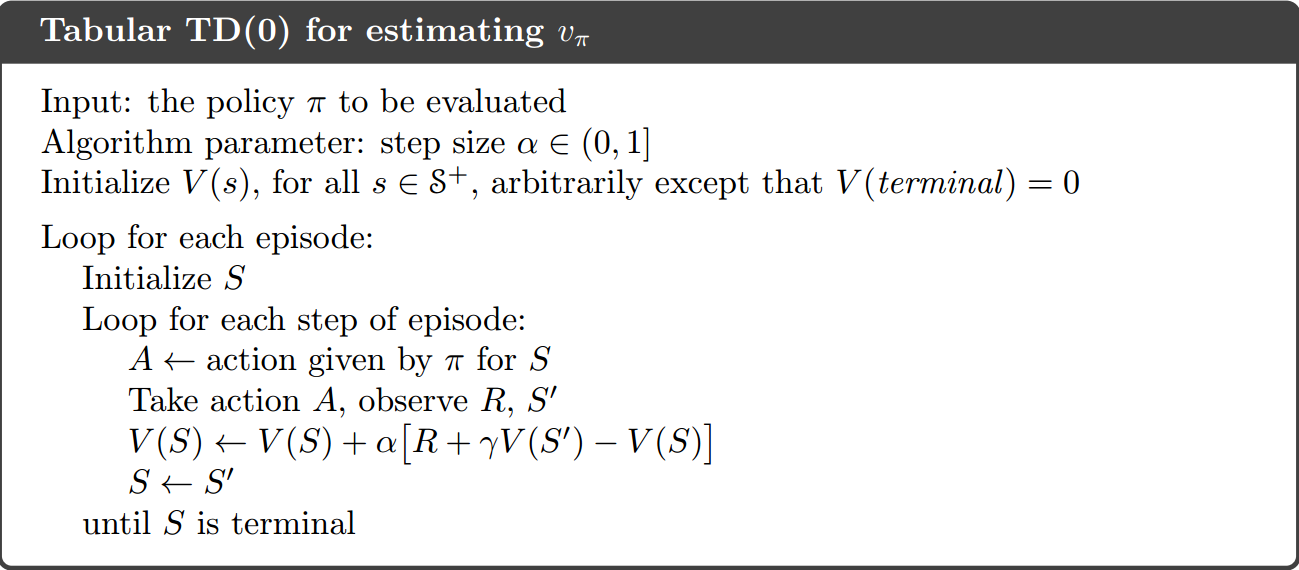
\includegraphics[scale = 0.3]{TD_0_algo.png}}
\end{minipage}
\caption{\footnotesize{\textbf{TD($0$) algorithm}}}
\label{fig: TD_0_algo}
\end{figure}

The Temporal-Difference (TD) learning extends the formula in \eqref{eqn: incremental_update} by replacing the new estimate/rewards  with the new estimates \underline{\emph{in next step}} and the rewards; $G_{t} = R_{t+1}+ \gamma  G_{t+1}$. Then TD replaces the estimate of cumulative rewards at $t+1$, $G_{t+1}$, with the value function $V(S_{t+1})$ at $t+1$
\begin{align}
V(S_{t}) &\leftarrow V(S_{t}) + \alpha_{t}\paren{G_{t} - V(S_{t})} \nonumber\\
&\approx V(S_{t}) + \alpha_{t}\paren{R_{t+1} + \gamma V(S_{t+1})  - V(S_{t})}. \label{eqn: incremental_update_td}
\end{align} This algorithm is called \textbf{\emph{one-step TD}} or \textbf{\emph{TD(0)}}. It is a special case of \emph{multi-step TD or TD($\lambda$)}. The approximation of target \underline{$G_{t} \approx R_{t+1} + \gamma V(S_{t+1})$} is the key for TD learning. It comes from Bellman equation combining with Monte Carlo estimation:
\begin{align}
v_{\pi}(s) &= \E{\pi}{G_{t} | S_{t} = s} \approx  \E{\text{emp}}{G_{t} | S_{t} = s}\nonumber\\
&=  \E{\pi}{ R_{t+1}+ \gamma G_{t+1} | S_{t} = s}\nonumber\\
&=\E{\pi}{R_{t+1}  + \gamma\,v_{\pi}(S_{t+1}) | S_{t} = s}, \text{ (Bellman equation)} \nonumber\\
&\approx \E{\text{emp}}{R_{t+1}  + \gamma\,v_{\pi}(S_{t+1}) | S_{t} = s}, \text{ (Monte Carlo estimate)} \nonumber\\
\text{thus }G_{t}&\approx R_{t+1}+  \gamma v_{\pi}(S_{t+1})\nonumber\\
&\approx R_{t+1}+  \gamma  V(S_{t+1}).
\end{align}The last approximation is to replace $v_{\pi}$ with its estimate $V$. Whereas Monte Carlo methods must wait until the \emph{end of the episode} to determine the increment to $V(S_t)$ (only then is $G_t$ known), TD methods need to wait only until the \emph{next time step}. The quantity \underline{$R_{t+1} + \gamma V(S_{t+1})$} is referred as the \emph{\textbf{target}} (instead of $G_{t}$ for Monte Carlo methods.) and $\underline{\delta_{t} := R_{t+1} + \gamma V(S_{t+1})  - V(S_{t})}$ as the Temporal-Difference error or, \textbf{\emph{TD error}}. Figure \ref{fig: TD_0_algo} shows the TD($0$) algorithm 

Let us compare TD learning  to Dynamic Programming (DP) and Monte Carlo (MC). Because TD($0$) bases its update in part on an existing estimate, we say that it is a
\emph{bootstrapping} method, like DP. Check the value function and Bellman equation as 
\begin{align}
\text{DP: }v_{\pi}(s) &=  \E{\pi}{R_{t+1}  + \gamma\,v_{\pi}(S_{t+1}) | S_{t} = s} \label{eqn: DP_target} \\
\text{MC: }v_{\pi}(s) &=  \E{\pi}{G_{t} | S_{t} = s}  \label{eqn: MC_target}
\end{align} DP estimate uses an estimate of the Bellman equation \eqref{eqn: DP_target} as target. Although the expectation can be computed exactly, the value at state $S_{t+1}$ is an estimate since we do not know $S_{t+1}$ at time $t$. The MC uses an estimate of \eqref{eqn: MC_target} as target. The Monte Carlo target is an estimate because the expected value is not known; a \emph{sample return} is used in place of the real expected return. The TD target is an estimate for \emph{both reasons}: it \emph{samples the expected values} in \eqref{eqn: DP_target} and it uses the current estimate $V$ instead of the true $v_{\pi}$. Thus, TD methods combine the \textbf{sampling} of Monte Carlo with the \textbf{bootstrapping} of DP.

\begin{figure}
\begin{minipage}[t]{0.3\linewidth}
  \centering
  \centerline{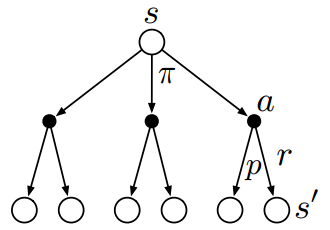
\includegraphics[scale = 0.3]{backup_diagram_dp.png}}
  \vspace{-7pt}
 \centerline{\footnotesize{(a) }}
\end{minipage}
\begin{minipage}[t]{0.3\linewidth}
  \centering
  \centerline{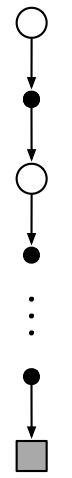
\includegraphics[scale = 0.3]{backup_diagram_mc.png}}
  \vspace{-7pt}
 \centerline{\footnotesize{(b) }}
\end{minipage}
\begin{minipage}[t]{0.3\linewidth}
  \centering
  \centerline{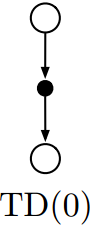
\includegraphics[scale = 0.3]{backup_diagram_td.png}}
  \vspace{-7pt}
 \centerline{\footnotesize{(c) }}
\end{minipage}
\caption{\footnotesize{\textbf{Backup diagram for (a) Dynamic Programming (DP); (b) Monte Carlo (MC) methods; (c) Temporal-Difference (TD(0)) learning. Note that both DP and TD used boostrapping to compute state-value based on previous estimate of state-value function. MC only updates at the end of episode.}}}
\label{fig: backup_diagram_dp_mc_td}
\end{figure}

Figure \ref{fig: backup_diagram_dp_mc_td} compare the update of DP, MC and TD in backup diagram. We see that both DP and TD replies on bootstrapping to compute estimate based on existing estimate. On the other hand, both MC and TD updates as \emph{sample updates} because they involve looking ahead to a \emph{sample successor state} (or state-action pair), using the value of the successor and the reward along the way to compute a backed-up value, and then updating the value of the original state (or state-action pair) accordingly. This is different from \emph{expected update} from DP, which uses the complete knowledge of dynamics $p$.

The TD-error $\delta_{t}$ measuring the difference between the \emph{estimated value} of $S_t$ and the \emph{better estimate}/target $R_{t+1} + \gamma V(S_{t+1})$. $\delta_{t}$ is the error of estimation in $V(S_{t})$, available at time $t + 1$. $\delta_{t}$ will not be available until $t+1$. 
\begin{align}
\delta_{t} := R_{t+1} + \gamma V(S_{t+1})  - V(S_{t}) \label{eqn: td_error}
\end{align} We can actually rewrite the error for Monte Carlo estimate using $\delta_{t}$
\begin{align*}
G_{t} -  V(S_{t}) &= R_{t+1} + \gamma G_{t+1} - V(S_{t}) +  \gamma V(S_{t+1}) -  \gamma V(S_{t+1})  \\
&= \delta_{t} +  \gamma \paren{G_{t+1} -V(S_{t+1})} \\
&=  \delta_{t} +   \gamma\delta_{t+1} + \gamma^2 \paren{G_{t+2} -V(S_{t+2})} \\
&\ldots\\
&= \sum_{k=t}^{T-1}\gamma^{t-k}\delta_{k}
\end{align*} If $S_{t+1}$ is terminal, then the TD-error is $\delta_{t} := R_{t+1}  - V(S_{t}) $ since $V(\text{terminal}) = 0$.

\subsection{Advantages of TD Prediction Methods}
\begin{figure}
\begin{minipage}[t]{1\linewidth}
  \centering
  \centerline{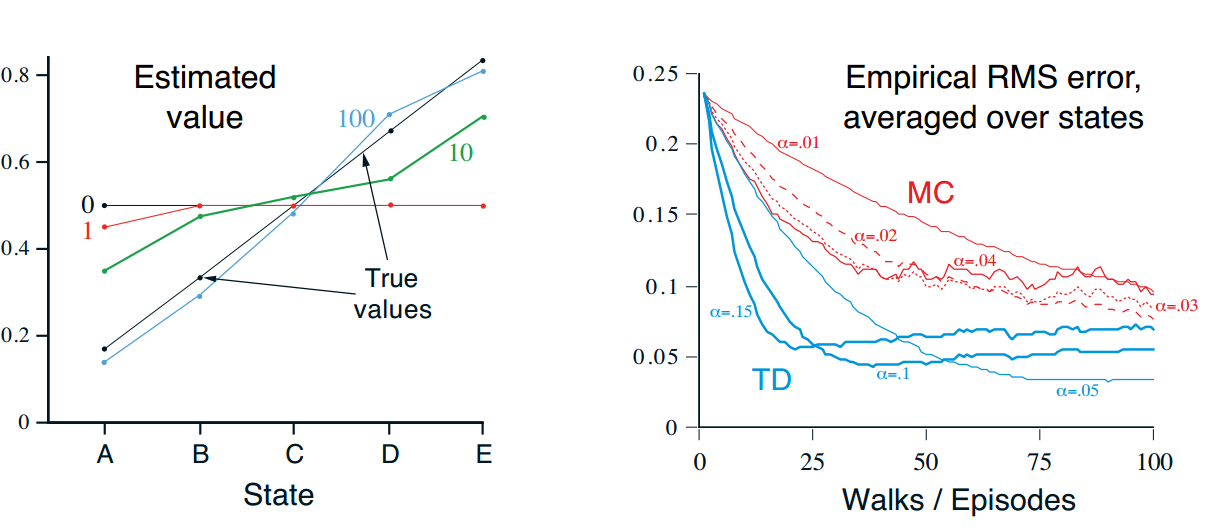
\includegraphics[scale = 0.3]{td_mc_example.png}}
\end{minipage}
\caption{\footnotesize{\textbf{An example from \citep{sutton2018reinforcement} based on random walk Markov decision process. It can be seen that TD converge faster than MC since it updates value estimate faster at each time step.}}}
\label{fig: td_mc_example}
\end{figure}
The advantages of temporal difference method TD(0) over dynamic programming and Monte Carlo methods can be summarized as below:
\begin{itemize}
\item Both Monte Carlo, TD(0) are \textbf{\emph{sample-based learning algorithm}}. They do not require complete knowledge of \emph{dynamics} $p$.  DP, however, requires a \emph{model}. 

\item TD($0$) learning naturally is an \textbf{\emph{online learning algorithm}}, which updates the value estimate at end of each time step. On the other hand, Monte Carlo algorithm only updates at\emph{ the end of episode} so that it can observe the return value. Because of this, TD($0$) updates information based on observed rewards faster than MC. MC is very \emph{slow} esp. when one episode is long. Some Monte Carlo methods must ignore or discount episodes on which experimental actions are taken, which can greatly slow learning.

\item TD(0) learning also has \emph{\textbf{convergence guarantee}}. For any fixed policy $\pi$, TD($0$) has been proved to converge to $v_{\pi}$, in the \emph{mean} for a constant step-size parameter if it is sufficiently small, and \emph{with probability $1$} if the step-size parameter decreases according to the usual stochastic approximation conditions. In that sense, both TD and Monte Carlo methods converge \emph{asymptotically} to the correct predictions. 

\item Both DP and TD(0) use \emph{\textbf{bootstrapping}}. They learn aguess from a guess, i.e. they update the value estimate of a state based on value estimate of its successor state plus the rewards after it. In other words, This helps to \emph{reduce the variance} of estimate compared to MC methods. 
\end{itemize}

We can also compare with unsupervised learning and supervised learning:
\begin{itemize}
\item Like MC and DP, TD prediction has a \emph{target}. On the other hand, all of these methods are \emph{\textbf{unsupervised}} since no human label is needed. Just need to wait for the target observation. In that sense, it is more \emph{scalable}, and \emph{model-free}. TD learning is a method for \emph{\textbf{learning to predict}}. In particular, it learns a prediction based on \emph{another, later, learned} prediction.  \textbf{TD error} is the difference between two predictions $R_{t+1} + \gamma V(S_{t+1})$ and $V(S_{t})$. In this sense, it is very similar to \textbf{supervised learning}. Like \emph{back-propagation the error} in supervised learning, TD learning also predict the value backwards from the terminal state. 

\item TD learning is relevent only when we consider \emph{\textbf{multi-step} prediction}.  The thing predicted (the discounted cumulative rewards conditional on some behavior) is multi-step in the future. This is very different from supervised learning, which makes a one-step prediction only. 
\end{itemize}

\section{Temporal-Difference Control}
\subsection{Sarsa: On-policy TD Control}
\begin{figure}
\begin{minipage}[t]{1\linewidth}
  \centering
  \centerline{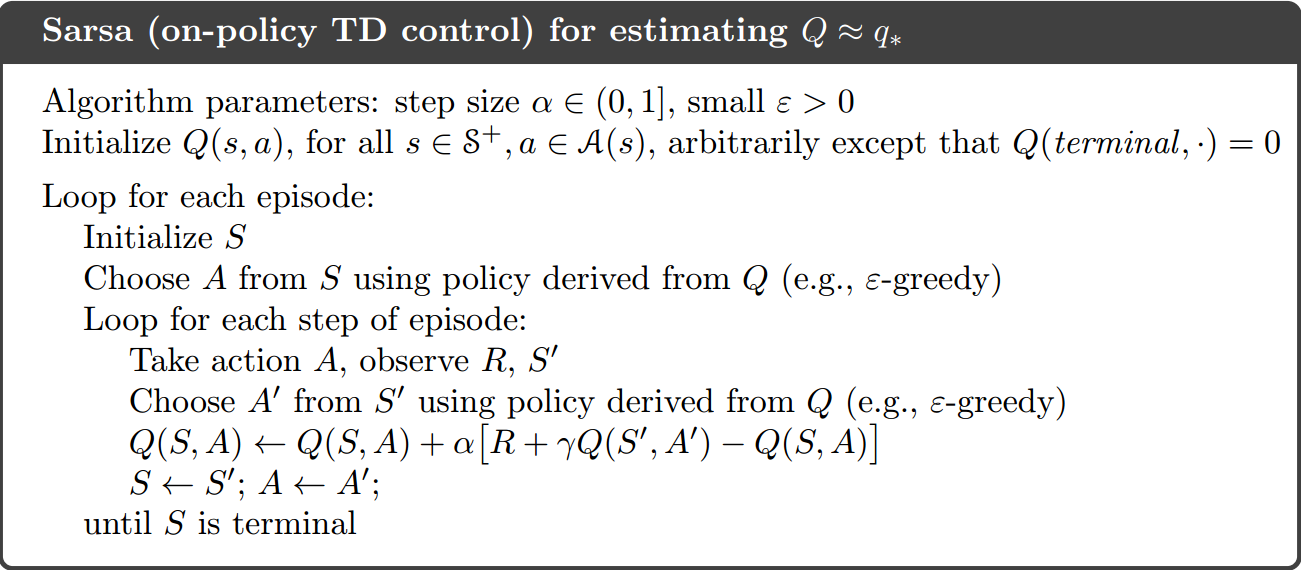
\includegraphics[scale = 0.3]{sarsa_control.png}}
\end{minipage}
\caption{\footnotesize{\textbf{Sarsa, on-policy TD control}}}
\label{fig: sarsa_control}
\end{figure}
TD prediction methods can be used for the control problem. Note that in Generalized Policy Iteration (GPI), the policy improvement is obtained by choosing greedy/$\epsilon$-greedy policy with respect to the action-value function. \emph{\textbf{Sarsa algorithm}} only substitute the TD methods for the evaluation or prediction part in the GPI.  
  
Since we need to estimate the action-value function using TD learning, we recall the Bellman equation for action-value function $q$ and state-value function $v$ as below. 
\begin{align}
v_{\pi}(s) &=  \E{\pi}{R_{t+1}  + \gamma\,v_{\pi}(S_{t+1}) | S_{t} = s}  \nonumber\\
q_{\pi}(s, a) &= \E{}{R_{t+1} + \gamma q_{\pi}(S_{t+1}, A_{t+1}) | S_{t}=s, A_{t}=a} \label{eqn: bellman_eqn_value_action2}
\end{align} Similar to how TD prediction is derived from the equation of state-value function, Sarsa derive the TD prediction from the equation of action-value function.
\begin{align}
V(S_{t}) &\leftarrow V(S_{t}) + \alpha_{t}\brac{R_{t+1} + \gamma V(S_{t+1})  - V(S_{t})}. \nonumber\\
Q(S_{t}, A_{t}) &\leftarrow Q(S_{t}, A_{t}) + \alpha_{t}\brac{R_{t+1} + \gamma Q(S_{t+1}, A_{t+1})  - Q(S_{t}, A_{t})}. \label{eqn: sarsa_predict}
\end{align}  As in \eqref{eqn: sarsa_predict}, we see that the estimate of state-value function $Q$ at time $t$ depends on the state-value function estimate at $t+1$, rewards at $t+1$. The name of \emph{Sarsa} comes from the fact that the update is controlled by the tuple $(S_{t}, A_{t}, R_{t+1}, S_{t+1}, A_{t+1})$. (unlike the TD prediction, here we need to sample a new action based on the new state and policy.)

Sarsa algorithm is on-policy control, since the policy used to generate actions is the same policy that is updated. As in all on-policy methods, we continually estimate $q_{\pi}$ for the behavior policy $\pi$, and at the same time change $\pi$ toward greediness with respect to $q_{\pi}$. The general form of the Sarsa control algorithm is given in the box on the next page. Like on-policy MC control, we have to balance the exploration-exploitation by choosing $\pi$ as $\epsilon$-soft. Figure \ref{fig: sarsa_control} describes the Sarsa algorithm. 

The convergence properties of the Sarsa algorithm depend on the nature of the policy’s dependence on $Q$. Using $\epsilon$-soft/$\epsilon$-greedy policy, Sarsa converges
with probability $1$ to an optimal policy and action-value function as long as all state–action pairs are visited an infinite number of times and the policy converges in the limit to the greedy policy.

\subsection{Q-learning: Off-policy TD Control}
\begin{figure}
\begin{minipage}[t]{1\linewidth}
  \centering
  \centerline{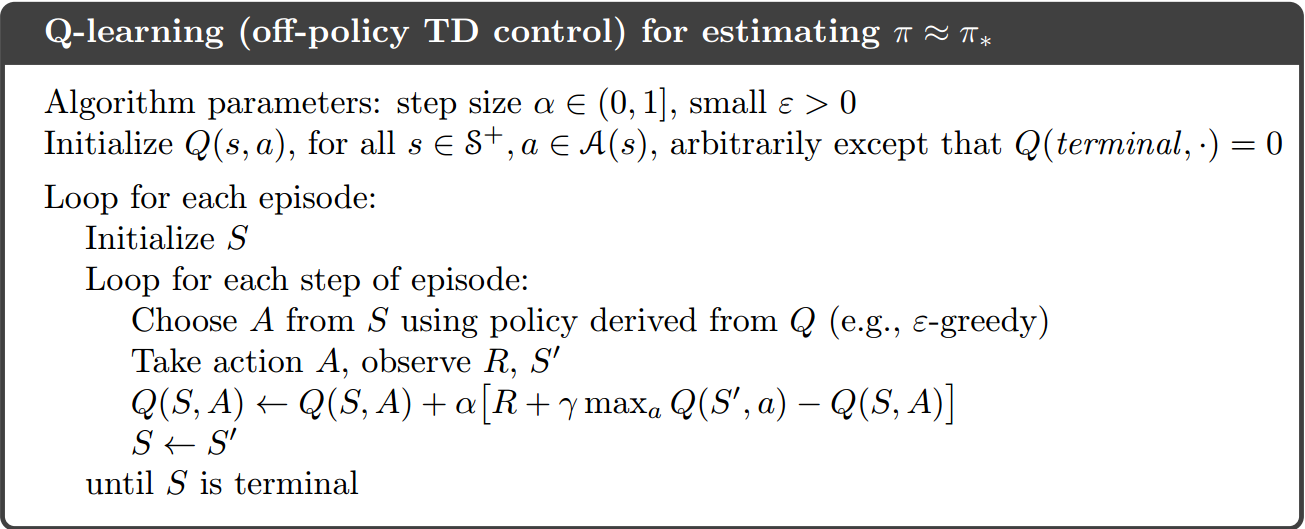
\includegraphics[scale = 0.3]{q_learning.png}}
\end{minipage}
\caption{\footnotesize{\textbf{Q-learning, off-policy TD control}}}
\label{fig: q_learning}
\end{figure}
One of the early breakthroughs in reinforcement learning was the development of an off-policy TD control algorithm known as \textbf{\emph{Q-learning}}.
 
Instead of Bellman equation for $q$, we now consider the Bellman optimality equation for $q_{*}$
\begin{align}
q_{\pi}(s, a) &= \E{}{R_{t+1} + \gamma q_{\pi}(S_{t+1}, A_{t+1}) | S_{t}=s, A_{t}=a} \nonumber\\
q_{*}(s, a) &= \E{}{R_{t+1} + \gamma  \max_{a'\in \cA(s)}q_{*}(S_{t+1}, a')  \Big| S_{t} = s, \, A_{t} = a}  \label{eqn: bellman_eqn_optimal_value_action3}
\end{align} The update rule for Q-learning is defined by
\begin{align}
Q(S_{t}, A_{t}) &\leftarrow Q(S_{t}, A_{t}) + \alpha_{t}\brac{R_{t+1} + \gamma \max_{a'\in \cA(S_{t+1})}Q(S_{t+1}, a')  - Q(S_{t}, A_{t})}. \label{eqn: q_learning}
\end{align}
As indicated in \eqref{eqn: bellman_eqn_optimal_value_action3}, the learned action-value function, $Q$, directly approximates $q_{*}$, the optimal
action-value function, independent of the policy being followed.  While Sarsa is a sample-based \emph{policy iteration algorithm}, the \emph{Q-learning} is a sample-based \textbf{\emph{value-iteration algorithm}}. 

Q-learning is an \emph{\textbf{off-policy control}} since the target policy learned does not depend on the policy used to generate new action $A_{t+1}$. In fact, $\max_{a'\in \cA(S_{t+1})}Q(S_{t+1}, a')$ implies that the \emph{target policy} is a deterministic greedy policy $\pi'(s) = \argmax_{a'}Q(S_{t+1}, a')$, whereas the behavior policy $\pi$ is stochastic like $\epsilon$-greedy. 

$Q$ approximates the optimal action value function independent of the behavior policy.  The behavior policy still has an effect in that it determines which state-action pairs are visited and updated. However, all that is required for \emph{correct convergence} is that all pairs continue to be updated. This is a \emph{minimal requirement} in the sense that any method guaranteed to find optimal behavior in the general case must require it. Under this assumption and a variant of the usual stochastic approximation conditions on the sequence of step-size parameters, Q has been shown to \textbf{converge with probability 1} to $q_{*}$. Figure \ref{eqn: q_learning} describes the Q-learning.



\subsection{Expected Sarsa: Off-policy TD Control}
\begin{figure}
\begin{minipage}[t]{0.3\linewidth}
  \centering
  \centerline{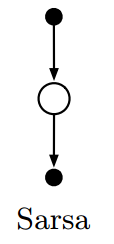
\includegraphics[scale = 0.3]{backup_diagram_sarsa.png}}
  \vspace{-7pt}
 \centerline{\footnotesize{(a) }}
\end{minipage}
\begin{minipage}[t]{0.3\linewidth}
  \centering
  \centerline{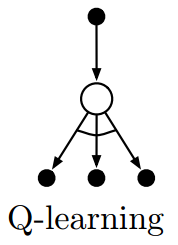
\includegraphics[scale = 0.3]{backup_diagram_q_learning.png}}
  \vspace{-7pt}
 \centerline{\footnotesize{(b) }}
\end{minipage}
\begin{minipage}[t]{0.3\linewidth}
  \centering
  \centerline{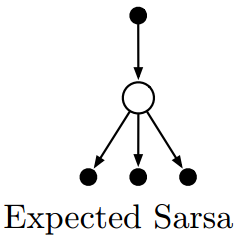
\includegraphics[scale = 0.3]{backup_diagram_exp_sarsa.png}}
  \vspace{-7pt}
 \centerline{\footnotesize{(c) }}
\end{minipage}
\caption{\footnotesize{\textbf{Backup diagram for (a) Sarsa; (b) Q-learning; (c) Expected Sarsa.}}}
\label{fig: backup_diagram_td_control}
\end{figure}

\textbf{\emph{Expected Sarsa}} is an algorithm derived from the same Bellman equation \eqref{eqn: bellman_eqn_value_action3} as the Sarsa. However, instead of sample the next action $A_{t+1}$, we can directly computed the exact expected value since we know policy $\pi(a'|\cdot), \forall\,a'$. Compare to Q-learning, we can replace the maximization in \eqref{eqn: q_learning} with the expectation. 

From the Bellman equation for action-valued function, 
\begin{align}
q_{\pi}(s, a) &= \E{}{R_{t+1} + \gamma q_{\pi}(S_{t+1}, A_{t+1}) | S_{t}=s, A_{t}=a} \nonumber\\
                    &=  \E{}{R_{t+1} + \gamma \sum_{a'}\pi(a'|S_{t+1})q_{\pi}(S_{t+1}, a') \Big| S_{t}=s, A_{t}=a} \label{eqn: bellman_eqn_value_action3}
\end{align}
\textbf{\emph{Expected Sarsa}} has the update rule as 
\begin{align}
Q(S_{t}, A_{t}) &\leftarrow Q(S_{t}, A_{t}) + \alpha_{t}\brac{R_{t+1} + \gamma\sum_{a'}\pi(a'|S_{t+1})Q(S_{t+1}, a')  - Q(S_{t}, A_{t})}. \label{eqn: expected_sarsa_predict}
\end{align} Expected Sarsa is an \textbf{off-policy control} since the update does not depend on the behavior policy that generates the new action since the expectation is computed for \emph{all} actions. Given the next state, $S_{t+1}$, this algorithm moves \emph{\textbf{deterministically}} in the same direction as Sarsa moves in \textbf{\emph{expectation}},

Expected Sarsa is more complex computationally than Sarsa but, in return, it \emph{eliminates the variance} due to the random selection of $A_{t+1}$. Given the same amount of experience we might expect it to perform slightly better than Sarsa, and indeed it generally does. By evaluating all actions instead of the maximal action, the expected Sarsa would choose actions more safely to avoid potential high loss when choosing the optimal action deterministically. 


\begin{figure}
\begin{minipage}[t]{1\linewidth}
  \centering
  \centerline{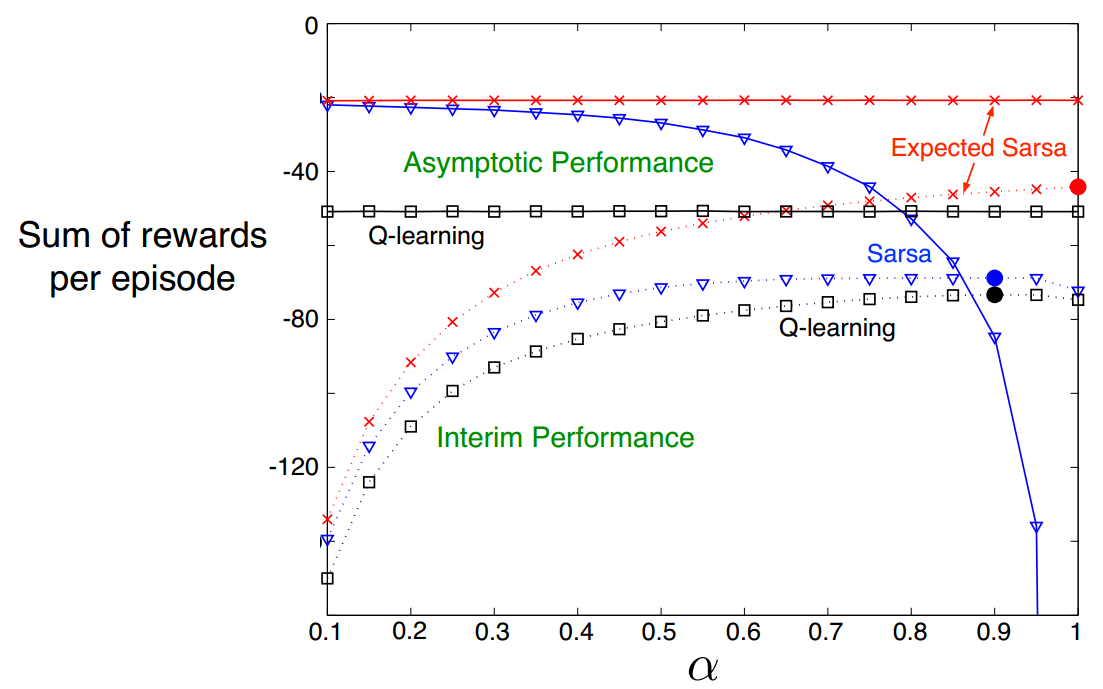
\includegraphics[scale = 0.3]{comp_q_sarsa_exp.png}}
\end{minipage}
\caption{\footnotesize{\textbf{Experiment performance between Sarsa, Q-learning, Expected Sarsa. Note that Sarsa is impacted by the choice of $\alpha$ but Q-learning and Expected Sarsa are not.}}}
\label{fig: q_learning}
\end{figure}

\section{Summary}
We can summarize the update rule for Sarsa, Q-learning and expected Sarsa as a simple update rule, using $\hat{G}_{t}$ as the approximate return at $t$: 
\begin{align*}
Q(S_{t}, A_{t}) &\leftarrow Q(S_{t}, A_{t}) + \alpha_{t}\brac{\hat{G}_{t}  - Q(S_{t}, A_{t})}.  \\
 \text{  \textbf{Sarsa} }\quad\hat{G}_{t} &= R_{t+1} + \gamma Q(S_{t+1}, A_{t+1}) \\
\text{  \textbf{Q-Learning} }\quad\hat{G}_{t} &=  R_{t+1} + \gamma \max_{a'\in \cA(S_{t+1})}Q(S_{t+1}, a')  \\
 \text{  \textbf{Expected Sarsa} }\quad\hat{G}_{t} &= R_{t+1} + \gamma\sum_{a'}\pi(a'|S_{t+1})Q(S_{t+1}, a') 
\end{align*} The \textbf{key} for TD Control compared to Monte Carlo Control is that  $\hat{G}_{t}$ is \emph{partially \textbf{computed}} instead of \emph{\textbf{observed}} from real experience only.  Note that TD Control need as much information from real experience as MC Control but is learning much faster. As compared to functional approximation, TD Control is also \emph{\textbf{cheap}} in terms of requirements on computational resources.  

\newpage
\bibliographystyle{plainnat}
\bibliography{reference.bib}
\end{document}